%% BioMed_Central_Tex_Template_v1.06
%%                                      %
%  bmc_article.tex            ver: 1.06 %
%                                       %

%%IMPORTANT: do not delete the first line of this template
%%It must be present to enable the BMC Submission system to
%%recognise this template!!

%%%%%%%%%%%%%%%%%%%%%%%%%%%%%%%%%%%%%%%%%
%%                                     %%
%%  LaTeX template for BioMed Central  %%
%%     journal article submissions     %%
%%                                     %%
%%          <8 June 2012>              %%
%%                                     %%
%%                                     %%
%%%%%%%%%%%%%%%%%%%%%%%%%%%%%%%%%%%%%%%%%


%%%%%%%%%%%%%%%%%%%%%%%%%%%%%%%%%%%%%%%%%%%%%%%%%%%%%%%%%%%%%%%%%%%%%
%%                                                                 %%
%% For instructions on how to fill out this Tex template           %%
%% document please refer to Readme.html and the instructions for   %%
%% authors page on the biomed central website                      %%
%% http://www.biomedcentral.com/info/authors/                      %%
%%                                                                 %%
%% Please do not use \input{...} to include other tex files.       %%
%% Submit your LaTeX manuscript as one .tex document.              %%
%%                                                                 %%
%% All additional figures and files should be attached             %%
%% separately and not embedded in the \TeX\ document itself.       %%
%%                                                                 %%
%% BioMed Central currently use the MikTex distribution of         %%
%% TeX for Windows) of TeX and LaTeX.  This is available from      %%
%% http://www.miktex.org                                           %%
%%                                                                 %%
%%%%%%%%%%%%%%%%%%%%%%%%%%%%%%%%%%%%%%%%%%%%%%%%%%%%%%%%%%%%%%%%%%%%%

%%% additional documentclass options:
%  [doublespacing]
%  [linenumbers]   - put the line numbers on margins

%%% loading packages, author definitions

\documentclass[twocolumn]{bmcart}% uncomment this for twocolumn layout and comment line below
%\documentclass{bmcart}

%%% Load packages
\usepackage{amsthm,amsmath}
%\RequirePackage{natbib}
\RequirePackage{hyperref}
\usepackage[utf8]{inputenc} %unicode support
\usepackage{graphicx}
\usepackage{cprotect}
\usepackage{listings}
\lstset{
basicstyle=\footnotesize\ttfamily,
columns=flexible,
breaklines=true,
breakatwhitespace=true,
aboveskip=3pt,
belowskip=3pt,
}
\allowdisplaybreaks[2]
%\usepackage[applemac]{inputenc} %applemac support if unicode package fails
%\usepackage[latin1]{inputenc} %UNIX support if unicode package fails


%%%%%%%%%%%%%%%%%%%%%%%%%%%%%%%%%%%%%%%%%%%%%%%%%
%%                                             %%
%%  If you wish to display your graphics for   %%
%%  your own use using includegraphic or       %%
%%  includegraphics, then comment out the      %%
%%  following two lines of code.               %%
%%  NB: These line *must* be included when     %%
%%  submitting to BMC.                         %%
%%  All figure files must be submitted as      %%
%%  separate graphics through the BMC          %%
%%  submission process, not included in the    %%
%%  submitted article.                         %%
%%                                             %%
%%%%%%%%%%%%%%%%%%%%%%%%%%%%%%%%%%%%%%%%%%%%%%%%%


%\def\includegraphic{}
%\def\includegraphics{}



%%% Put your definitions there:
\startlocaldefs
\endlocaldefs


%%% Begin ...
\begin{document}

%%% Start of article front matter
\begin{frontmatter}

\begin{fmbox}
\dochead{Software}

%%%%%%%%%%%%%%%%%%%%%%%%%%%%%%%%%%%%%%%%%%%%%%
%%                                          %%
%% Enter the title of your article here     %%
%%                                          %%
%%%%%%%%%%%%%%%%%%%%%%%%%%%%%%%%%%%%%%%%%%%%%%

\title{Software for the analysis and visualization of deep mutational scanning data}

%%%%%%%%%%%%%%%%%%%%%%%%%%%%%%%%%%%%%%%%%%%%%%
%%                                          %%
%% Enter the authors here                   %%
%%                                          %%
%% Specify information, if available,       %%
%% in the form:                             %%
%%   <key>={<id1>,<id2>}                    %%
%%   <key>=                                 %%
%% Comment or delete the keys which are     %%
%% not used. Repeat \author command as much %%
%% as required.                             %%
%%                                          %%
%%%%%%%%%%%%%%%%%%%%%%%%%%%%%%%%%%%%%%%%%%%%%%

\author[
   addressref={aff1},                   % id's of addresses, e.g. {aff1,aff2}
   corref={aff1},                       % id of corresponding address, if any
   email={jbloom@fredhutch.org}   % email address
]{\inits{JD}\fnm{Jesse D.} \snm{Bloom}}


%%%%%%%%%%%%%%%%%%%%%%%%%%%%%%%%%%%%%%%%%%%%%%
%%                                          %%
%% Enter the authors' addresses here        %%
%%                                          %%
%% Repeat \address commands as much as      %%
%% required.                                %%
%%                                          %%
%%%%%%%%%%%%%%%%%%%%%%%%%%%%%%%%%%%%%%%%%%%%%%

\address[id=aff1]{%                           % unique id
  \orgname{Division of Basic Sciences and Computational Biology Program, Fred Hutchinson Cancer Research Center}, % university, etc
  \street{1100 Fairview Ave N},                     %
  \postcode{98109}                                % post or zip code
  \city{Seattle, WA},                              % city
  \cny{USA}                                    % country
}


%%%%%%%%%%%%%%%%%%%%%%%%%%%%%%%%%%%%%%%%%%%%%%
%%                                          %%
%% Enter short notes here                   %%
%%                                          %%
%% Short notes will be after addresses      %%
%% on first page.                           %%
%%                                          %%
%%%%%%%%%%%%%%%%%%%%%%%%%%%%%%%%%%%%%%%%%%%%%%

\begin{artnotes}
%\note{Sample of title note}     % note to the article
%\note[id=n1]{Equal contributor} % note, connected to author
\end{artnotes}

\end{fmbox}% comment this for two column layout

%%%%%%%%%%%%%%%%%%%%%%%%%%%%%%%%%%%%%%%%%%%%%%
%%                                          %%
%% The Abstract begins here                 %%
%%                                          %%
%% Please refer to the Instructions for     %%
%% authors on http://www.biomedcentral.com  %%
%% and include the section headings         %%
%% accordingly for your article type.       %%
%%                                          %%
%%%%%%%%%%%%%%%%%%%%%%%%%%%%%%%%%%%%%%%%%%%%%%

\begin{abstractbox}

\begin{abstract} % abstract
\parttitle{Background} %if any
Deep mutational scanning is a technique to estimate the impacts of mutations on a gene by using deep sequencing to count mutations in a library of variants before and after imposing a functional selection. The impacts of mutations must be inferred from changes in their counts after selection.

\parttitle{Results} %if any
I describe a software package, \texttt{dms\_tools}, to infer the impacts of mutations from deep mutational scanning data using a likelihood-based treatment of the mutation counts. I show that \texttt{dms\_tools} yields more accurate inferences on simulated data than the widely used but statistically biased approach of calculating ratios of counts pre- and post-selection. Using \texttt{dms\_tools}, one can infer the preference of each site for each amino acid given a single selection pressure, or assess the extent to which these preferences change under different selection pressures. The preferences and their changes can be intuitively visualized with sequence-logo-style plots created using an extension to \texttt{weblogo}.

\parttitle{Conclusions}
\texttt{dms\_tools} implements a statistically principled approach for the analysis and subsequent visualization of deep mutational scanning data.
\end{abstract}

%%%%%%%%%%%%%%%%%%%%%%%%%%%%%%%%%%%%%%%%%%%%%%
%%                                          %%
%% The keywords begin here                  %%
%%                                          %%
%% Put each keyword in separate \kwd{}.     %%
%%                                          %%
%%%%%%%%%%%%%%%%%%%%%%%%%%%%%%%%%%%%%%%%%%%%%%

\begin{keyword}
\kwd{deep mutational scanning}
\kwd{sequence logo}
\kwd{amino-acid preferences}
\end{keyword}

% MSC classifications codes, if any
%\begin{keyword}[class=AMS]
%\kwd[Primary ]{}
%\kwd{}
%\kwd[; secondary ]{}
%\end{keyword}

\end{abstractbox}
%
%\end{fmbox}% uncomment this for twcolumn layout

\end{frontmatter}

%%%%%%%%%%%%%%%%%%%%%%%%%%%%%%%%%%%%%%%%%%%%%%
%%                                          %%
%% The Main Body begins here                %%
%%                                          %%
%% Please refer to the instructions for     %%
%% authors on:                              %%
%% http://www.biomedcentral.com/info/authors%%
%% and include the section headings         %%
%% accordingly for your article type.       %%
%%                                          %%
%% See the Results and Discussion section   %%
%% for details on how to create sub-sections%%
%%                                          %%
%% use \cite{...} to cite references        %%
%%  \cite{koon} and                         %%
%%  \cite{oreg,khar,zvai,xjon,schn,pond}    %%
%%  \nocite{smith,marg,hunn,advi,koha,mouse}%%
%%                                          %%
%%%%%%%%%%%%%%%%%%%%%%%%%%%%%%%%%%%%%%%%%%%%%%

%%%%%%%%%%%%%%%%%%%%%%%%% start of article main body
% <put your article body there>

%%%%%%%%%%%%%%%%
%% Background %%
%%

\section*{Background}
Deep mutational scanning is a high-throughput experimental technique to assess the impacts of mutations on a protein-coding gene~\cite{fowler2014deep}. Figure \ref{fig:DeepMutationalScan} shows a schematic of deep mutational scanning. A gene is mutagenized, and the library of resulting variants is introduced into cells or viruses, which are then subjected to an experimental selection that enriches for functional variants and depletes non-functional ones. Deep sequencing of the variants pre- and post-selection provides information about the functional impacts of mutations. Since the original description of deep mutational scanning by Fowler \textit{et al}~\cite{fowler2010high}, the technique has been applied to a wide range of genes~\cite{traxlmayr2012construction,mclaughlin2012spatial,starita2013activity,melamed2013deep,roscoe2013analyses,firnberg2014comprehensive,bloom2014experimentally,melnikov2014comprehensive,thyagarajan2014inherent,wu2014high,wu2014ns,olson2014comprehensive}, both to measure mutational tolerance given a single selection pressure as in Figure \ref{fig:DeepMutationalScan}A, or to identify mutations that have different effects under alternative selections as in Figure \ref{fig:DeepMutationalScan}B. New techniques to create comprehensive codon-mutant libraries of genes make it possible to profile all single amino-acid mutations~\cite{firnberg2012,jain2013rapid,firnberg2014comprehensive,bloom2014experimentally,melnikov2014comprehensive}, while new techniques for \textit{in vivo} mutagenesis enable deep mutational scanning to be applied across the biological spectrum from viruses and bacteria to human cells~\cite{findlay2014saturation}.

A key component of deep mutational scanning is analysis of the data: First, raw reads from the deep sequencing must be processed to count mutations pre- and post-selection. Next, the biological effects of mutations must be inferred from these counts. The first task of processing the reads is idiosyncratic to the specific sequencing strategy used. But the second task of inferring mutational effects from sequencing counts is amenable to more general algorithms. However, only a few such algorithms have been described~\cite{fowler2011enrich,bank2014bayesian}. Here I present user-friendly software, \texttt{dms\_tools}, that infers mutational effects from sequencing counts. Before describing the algorithms implemented in \texttt{dms\_tools} and illustrating its use on existing and simulated data, I first discuss issues associated with inferring mutational effects from sequencing counts.

\subsection*{The nature of deep mutational scanning data.}
The data consist of counts of variants pre- and post-selection. The approach presented here treats each site in the gene separately, ignoring epistatic coupling among mutations. This aspect of the approach should not be construed as a suggestion that interactions among mutations are unimportant; indeed, several studies have used deep mutational scanning to examine pairwise epistasis~\cite{olson2014comprehensive,araya2012fundamental,bank2015systematic}, and techniques have been described to obtain linkage between distant sites~\cite{hiatt2010parallel,wu2014hiv}. However, the exploding combinatorics of multiple mutations (a 500-residue protein has only $19 \times 500 \approx 10^4$ single mutants, but $19^2 \times \frac{500 \times 499}{2} \approx 4 \times 10^7$  double mutants and $19^3 \times \frac{500!}{497! \times 3!} \approx 10^{11}$ triple mutants) make it currently plausible to comprehensively characterize only single mutations to all but the shortest genes. Therefore, treating sites independently is not a major limitation for most current datasets; eventually the approach here might be extended to include coupling among mutations.

The data for each site $r$ is characterized by the sequencing \emph{depth} (total number of counts); let $N_r^{\rm{pre}}$, $N_r^{\rm{post}}$, $N_r^{s1}$, and $N_r^{s2}$ denote the depth at $r$ for each of the four libraries in Figure \ref{fig:DeepMutationalScan}. Typical depths for current experiments are $N \sim 10^6$. Denote the counts of character $x$ (characters might be nucleotides, amino acids, or codons) at $r$ as $n_{r,x}^{\rm{pre}}$, $n_{r,x}^{\rm{post}}$, $n_{r,x}^{s1}$, and $n_{r,x}^{s2}$. The values of $n_{r,x}$ for characters $x$ that differ from the wildtype identity $\operatorname{wt}\left(r\right)$ depend on both the depth $N$ and the average per-site mutation rate. Typical experiments introduce about one mutation per gene, so $\overline{\mu} \sim 1/L$ where $L$ is the length of the gene. Therefore, if a 500-codon gene is sequenced at depth $N \sim 10^6$, we expect $N \overline{\mu} \sim 2000$ counts of non-wildtype codons at each site. Since there are 63 mutant codons, the average pre-selection counts for a mutation to a specific $x \ne \operatorname{wt}\left(r\right)$ will be $n_{r,x}^{\rm{pre}} \sim 30$, with counts for most mutations deviating from this average due to biases in creation of the mutant library and randomness in which molecules are sequenced. Counts in the post-selection libraries will further deviate from this average due to selection. Therefore, even at depths $N \sim 10^6$, the actual counts of most mutations will be quite modest.

\subsection*{The challenge of statistical inference from finite counts.}
The goal is to estimate the effects of mutations from changes in their counts after selection. Let $\mu_{r,x}$, $f_{r,x}$, $f_{r,x}^{s1}$, and $f_{r,x}^{s2}$ denote the \emph{true} frequencies of $x$ at $r$ that would be observed for the four libraries in Figure \ref{fig:DeepMutationalScan} if we sampled at infinite depth in both the actual experiment and the sequencing. If we knew these frequencies, we could calculate parameters that reflect the effects of mutations. One parameter that characterizes the effect of mutating $r$ from $\operatorname{wt}\left(r\right)$ to $x$ for the experiment in Figure \ref{fig:DeepMutationalScan}A is the \emph{enrichment ratio}
\begin{equation}
\label{eq:enrichment}
\phi_{r,x} = \frac{f_{r,x} / f_{r,\operatorname{wt}\left(r\right)}}{\mu_{r,x} / \mu_{r,\operatorname{wt}\left(r\right)}}.
\end{equation}
Beneficial mutations have $\phi_{r,x} > 1$, while deleterious ones have $\phi_{r,x} < 1$. A related parameter is the \emph{preference} $\pi_{r,x}$ of $r$ for $x$. At each site, the preferences are simply the enrichment ratios rescaled to sum to one:
\begin{equation}
\label{eq:preference}
\pi_{r,x} = \frac{\phi_{r,x}}{\sum_y \phi_{r,y}} = \frac{f_{r,x} / \mu_{r,x}}{\sum_y f_{r,y} / \mu_{r,y}},
\end{equation}
or equivalently
\begin{equation}
\label{eq:preference2}
f_{r,x} = \frac{\pi_{r,x} \times \mu_{r,x}}{\sum_y \pi_{r,y} \times \mu_{r,y}}.
\end{equation}
The preferences can be intuitively visualized (Figure \ref{fig:DeepMutationalScan}A) and interpreted as the equilibrium frequencies in substitution models for gene evolution~\cite{bloom2014experimentally,bloom2014informed} (after accounting for uneven mutational rates~\cite{yampolsky2005exchangeability,stoltzfus2009climbing}). 

Equations \ref{eq:enrichment} and \ref{eq:preference} are in terms of the true frequencies $\mu_{r,x}$, $f_{r,x}$, etc. But in practice, we only observe the counts in the finite sample of sequenced molecules. The computational challenge is to estimate the preferences (or enrichment ratios) from these counts.

The most naive approach is to simply substitute the counts for the frequencies, replacing Equation \ref{eq:enrichment} with
\begin{equation}
\label{eq:enrichmentcounts}
\phi_{r,x} = \frac{\frac{n_{r,x}^{\rm{post}} + \mathcal{P}}{n_{r,\operatorname{wt}\left(r\right)}^{\rm{post}} + \mathcal{P}}}{\frac{n_{r,x}^{\rm{pre}} + \mathcal{P}}{n_{r,\operatorname{wt}\left(r\right)}^{\rm{pre}} + \mathcal{P}}}
\end{equation}
where $\mathcal{P}$ (often chosen to be one) is a pseudocount added to each count to avoid ratios of zero or infinity.

However, Equation \ref{eq:enrichmentcounts} involves ratios of counts with values $\sim 10$ to 100 -- and as originally noted by Karl Pearson~\cite{pearson1896mathematical,pearson1910}, ratios estimated from finite counts are statistically biased, with the bias increasing as the magnitude of the counts decrease. This bias can propagate into subsequent analyses, since many statistical tests assume symmetric errors. The problems caused by biases in uncorrected ratios have been noted even in applications such as isotope-ratio mass spectrometry~\cite{ogliore2011} and fluorescent imaging~\cite{van2000mean}, where the counts usually far exceed those in deep mutational scanning.

Taking ratios also abrogates our ability to use the magnitude of the counts to assess our certainty about conclusions. For instance, imagine that at a fixed depth, the counts of a mutation increase from a pre-selection value of 5 to a post-selection value of 10. While this doubling suggests that the mutation might be beneficial, the small counts make us somewhat uncertain of this conclusion. But if the counts increased from 20 to 40 we would be substantially more certain, and if they increased from 100 to 200 we would be quite sure. So only by an explicit statistical treatment of the counts can we fully leverage the data.

Here I describe a software package, \texttt{dms\_tools}, that infers mutational effects in a Bayesian framework using a likelihood-based treatment of the counts. This software can be used to infer and visualize site-specific preferences from experiments like Figure \ref{fig:DeepMutationalScan}A, and to infer and visualize differences in preferences under alternative selections from experiments like Figure \ref{fig:DeepMutationalScan}B. 

\section*{Implementation and Results}

\subsection*{Algorithm to infer site-specific preferences.}
\texttt{dms\_tools} uses a Bayesian approach to infer site-specific preferences from experiments like those in Figure \ref{fig:DeepMutationalScan}A. The algorithm calculates the likelihoods of the counts given the unknown preferences and mutation / error rates, placing plausible priors over these unknown parameters. The priors correspond to the assumption that all possible identities (e.g. amino acids) have equal preferences, and that the mutation and error rates for each site are equal to the overall average for the gene. MCMC is used to calculate the posterior probability of the preferences given the counts.

This algorithm a slight modification of that in the \textsl{Methods} of \cite{bloom2014experimentally}; here the algorithm is described anew to explain the implementation in \texttt{dms\_tools}. 

\subsubsection*{Optional controls to quantify error rates.}
Some sequencing reads that report a mutation may actually reflect an error. Errors can be quantified by sequencing an unmutated gene, so that any counts at $r$ of $x \ne \operatorname{wt}\left(r\right)$ for this control reflect errors. In some cases (e.g. sequencing an RNA virus where the post-selection libraries must be reverse-transcribed), error rates for the pre- and post-selection libraries may differ and so be described by different controls. Let $N_r^{\textrm{errpre}}$ and $N_r^{\rm{errpost}}$ be the depth and $n_{r,x}^{\rm{errpre}}$ and $n_{r,x}^{\rm{errpost}}$ be the counts of $x$ in the pre-selection and post-selection error controls, respectively. Define $\epsilon_{r,x}$ and $\rho_{r,x}$ to be the true frequencies of errors at $r$ from $\operatorname{wt}\left(r\right)$ to $x$ in the pre- and post-selection controls, respectively. 

\subsubsection*{Likelihoods of observing specific mutational counts.}
Define vectors of the counts and frequencies for all characters at each site $r$, i.e. $\mathbf{n_r^{\textbf{pre}}}= \left(\cdots, n_{r,x}^{\textrm{pre}}, \cdots\right)$, $\mathbf{n_r^{\textbf{post}}}= \left(\cdots, n_{r,x}^{\textrm{post}}, \cdots\right)$, $\boldsymbol{\mathbf{\mu_r}} = \left(\cdots, \mu_{r,x}, \cdots\right)$, $\boldsymbol{\mathbf{f_r}} = \left(\cdots, f_{r,x}, \cdots\right)$, etc. Also define $\boldsymbol{\mathbf{\pi_r}}= \left(\cdots, \pi_{r,x}, \cdots\right)$ of the preferences for each $r$, noting that Equation \ref{eq:preference2} implies $\boldsymbol{\mathbf{f_r}} = \frac{\boldsymbol{\mathbf{\mu_r}}\circ\boldsymbol{\mathbf{\pi_r}}}{\boldsymbol{\mathbf{\mu_r}}\cdot \boldsymbol{\mathbf{\pi_r}}}$ where $\circ$ is the Hadamard product.

The likelihoods of some specific set of counts are:
\begin{gather}
\begin{split} \Pr&\left(\mathbf{n_r^{\textbf{errpre}}} \mid N_r^{\textrm{errpre}}, \boldsymbol{\mathbf{\epsilon_r}}\right) = \\& \operatorname{Multi}\left(\mathbf{n_r^{\textbf{errpre}}}; N_r^{\textrm{errpre}}, \boldsymbol{\mathbf{\epsilon_r}}\right) \label{eq:pr_nrerrpre} \end{split} \\
\begin{split} \Pr&\left(\mathbf{n_r^{\textbf{errpost}}} \mid N_r^{\textrm{errpost}}, \boldsymbol{\mathbf{\rho_r}}\right) = \\ & \operatorname{Multi}\left(\mathbf{n_r^{\textbf{errpost}}}; N_r^{\textrm{errpost}}, \boldsymbol{\mathbf{\rho_r}}\right) \label{eq:pr_nrerrpost} \end{split} \\
\begin{split} \Pr&\left(\mathbf{n_r^{\textbf{pre}}}\mid N_r^{\textrm{pre}}, \boldsymbol{\mathbf{\mu_r}}, \boldsymbol{\mathbf{\epsilon_r}}\right) = \\ &\operatorname{Multi}\left(\mathbf{n_r^{\textbf{pre}}}; N_r^{\textrm{pre}}, \boldsymbol{\mathbf{\mu_r}}+ \boldsymbol{\mathbf{\epsilon_r}}- \boldsymbol{\mathbf{\delta_r}}\right) \label{eq:pr_nrpre} \end{split} \\
\begin{split} \Pr&\left(\mathbf{n_r^{\textbf{post}}} \mid N_r^{\textrm{post}}, \boldsymbol{\mathbf{\mu_r}}, \boldsymbol{\mathbf{\pi_r}}, \boldsymbol{\mathbf{\rho_r}}\right) = \\ &\operatorname{Multi}\left(\mathbf{n_r^{\textbf{post}}}; N_r^{\textrm{post}}, \frac{\boldsymbol{\mathbf{\mu_r}}\circ \boldsymbol{\mathbf{\pi_r}}}{\boldsymbol{\mathbf{\mu_r}}\cdot \boldsymbol{\mathbf{\pi_r}}} + \boldsymbol{\mathbf{\rho_r}}- \boldsymbol{\mathbf{\delta_r}}\right)\label{eq:pr_nrpost} \end{split}
\end{gather}
where $\operatorname{Multi}$ is the multinomial distribution, $\boldsymbol{\mathbf{\delta_r}} = \left(\cdots, \delta_{x, \operatorname{wt}\left(r\right)}, \cdots\right)$ is a vector with the element corresponding to $\operatorname{wt}\left(r\right)$ equal to one and all other elements zero ($\delta_{xy}$ is the Kronecker delta), and we have assumed that the probability that a site experiences both a mutation and an error is negligibly small.

\subsubsection*{Priors over the unknown parameters.}
We specify Dirichlet priors over the parameter vectors:
\begin{gather}
\Pr\left(\boldsymbol{\mathbf{\pi_r}}\right) = \operatorname{Dirichlet}\left(\boldsymbol{\mathbf{\pi_r}}; \alpha_{\pi} \times \mathbf{1}\right)   \label{eq:pr_pir} \\
\Pr\left(\boldsymbol{\mathbf{\mu_r}}\right) = \operatorname{Dirichlet}\left(\boldsymbol{\mathbf{\mu_r}}; \alpha_{\mu} \times \mathcal{N}_x \times \boldsymbol{\mathbf{a_{r,\mu}}}\right) \label{eq:pr_mur} \\
\Pr\left(\boldsymbol{\mathbf{\epsilon_r}}\right) = \operatorname{Dirichlet}\left(\boldsymbol{\mathbf{\epsilon_r}}; \alpha_{\epsilon} \times \mathcal{N}_x \times \boldsymbol{\mathbf{a_{r,\epsilon}}}\right) \label{eq:pr_epsilonr} \\
\Pr\left(\boldsymbol{\mathbf{\rho_r}}\right) = \operatorname{Dirichlet}\left(\boldsymbol{\mathbf{\rho_r}}; \alpha_{\rho} \times \mathcal{N}_x \times
 \boldsymbol{\mathbf{a_{r,\rho}}}\right) \label{eq:pr_rhor}
\end{gather}
where $\mathbf{1}$ is a vector of ones, $\mathcal{N}_x$ is the number of characters (64 for codons, 20 for amino acids, 4 for nucleotides), the $\alpha$'s are scalar concentration parameters $> 0$ (by default \texttt{dms\_tools} sets the $\alpha$'s to one). For codons, the error rate depends on the number of nucleotides being changed. The average error rates  $\overline{\epsilon_m}$ and $\overline{\rho_m}$ for $m$ nucleotide changes are estimated as
\begin{gather}
\overline{\epsilon_m} = \frac{1}{L}\sum\limits_r \frac{1}{N_r^{\textrm{errpre}}}\sum\limits_{x} n_{r,x}^{\textrm{errpre}}\times \delta_{m,D_{x,\operatorname{wt}\left(r\right)}} \label{eq:avgepsilonm} \\
\overline{\rho_m} = \frac{1}{L}\sum\limits_r \frac{1}{N_r^{\textrm{errpost}}}\sum\limits_{x} n_{r,x}^{\textrm{errpost}}\times \delta_{m,D_{x,\operatorname{wt}\left(r\right)}} \label{eq:avgrhom}
\end{gather}
where $D_{x,\operatorname{wt}\left(r\right)}$ is the number of nucleotide differences between $x$ and $\operatorname{wt}\left(r\right)$. Given these definitions, 
\begin{gather}
\boldsymbol{\mathbf{a_{r,\epsilon}}} = \left(\cdots, \sum\limits_m \frac{\overline{\epsilon}_{m}}{\mathcal{C}_m} \times \delta_{m,D_{x,\operatorname{wt}\left(r\right)}},\cdots\right) \label{eq:arepsilon} \\
\boldsymbol{\mathbf{a_{r,\rho}}} = \left(\cdots, \sum\limits_m \frac{\overline{\rho}_{m}}{\mathcal{C}_m} \times \delta_{m,D_{x,\operatorname{wt}\left(r\right)}}, \cdots\right) \label{eq:arrho} 
\end{gather}
where $\mathcal{C}_m$ is the number of mutant characters with $m$ changes relative to wildtype (for nucleotides $\mathcal{C}_0 = 1$ and $\mathcal{C}_1 = 3$; for codons $\mathcal{C}_0 = 1$, $\mathcal{C}_1 = 9$, $\mathcal{C}_2 = \mathcal{C}_3 = 27$).

Our prior assumption is that the mutagenesis introduces all mutant characters at equal frequency (this assumption is only plausible for codons if the mutagenesis is at the codon level as in~\cite{firnberg2012,jain2013rapid,firnberg2014comprehensive,bloom2014experimentally,melnikov2014comprehensive}). The per-site mutagenesis rate is estimated as
\begin{equation}
\label{eq:avgmu}
\overline{\mu} = \left(\frac{1}{L}\sum\limits_r \frac{1}{N_r^{\textrm{pre}}}\sum\limits_{x\ne \operatorname{wt}\left(r\right)} n_{r,x}^{\textrm{pre}}\right) - \sum\limits_{m \ge 1} \overline{\epsilon_m},
\end{equation}
so that
\begin{equation}
\boldsymbol{\mathbf{a_{r,\mu}}} = \left(\cdots, \frac{\overline{\mu}}{\mathcal{N}_x - 1} + \delta_{x,\operatorname{wt}\left(r\right)} \times \left[1 - \overline{\mu}\right] ,\cdots\right). \label{eq:armu}
\end{equation}

\subsubsection*{Character types: nucleotides, amino acids, or codons.}
\texttt{dms\_tools} allows four possibilities for the type of character for the counts and preferences. The first three possibilities are simple: the counts and preferences can both be for any of nucleotides, amino acids, or codons. 

The fourth possibility is that the counts are for codons, but the preferences for amino acids. In this case, define a function mapping codons to amino acids, 
\begin{equation}
\label{eq:A}
\mathbf{A}\left(\mathbf{w}\right) = \left(\cdots, \sum\limits_x \delta_{a,\mathcal{A}\left(x\right)} \times w_x, \cdots\right)
\end{equation}
where $\mathbf{w}$ is a 64-element vector of codons $x$, $\mathbf{A}\left(\mathbf{w}\right)$ is a 20- or 21-element (depending on the treatment of stop codons) vector of amino acids $a$, and $\mathcal{A}\left(x\right)$ is the amino acid encoded by $x$. The prior over the preferences $\boldsymbol{\mathbf{\pi_r}}$ is still a symmetric Dirichlet (now only of length 20 or 21), but the priors for $\boldsymbol{\mathbf{\mu_r}}$, $\boldsymbol{\mathbf{\epsilon_r}}$, and $\boldsymbol{\mathbf{\rho_r}}$ are now Dirichlets parameterized by $\mathbf{A}\left(\boldsymbol{\mathbf{a_{r,\mu}}}\right)$, $\mathbf{A}\left(\boldsymbol{\mathbf{a_{r,\epsilon}}}\right)$ and $\mathbf{A}\left(\boldsymbol{\mathbf{a_{r,\rho}}}\right)$ rather than $\boldsymbol{\mathbf{a_{r,\mu}}}$, $\boldsymbol{\mathbf{a_{r,\epsilon}}}$, and $\boldsymbol{\mathbf{a_{r,\rho}}}$. The likelihoods are computed in terms of these transformed vectors after similarly transforming the counts to $\mathbf{A}\left(\mathbf{n_r^{\textbf{pre}}}\right)$, $\mathbf{A}\left(\mathbf{n_r^{\textbf{post}}}\right)$, $\mathbf{A}\left(\mathbf{n_r^{\textbf{errpre}}}\right)$, and $\mathbf{A}\left(\mathbf{n_r^{\textbf{errpost}}}\right)$.

\subsubsection*{Implementation.}
The program \texttt{dms\_inferprefs} in the \texttt{dms\_tools} package infers the preferences by using \texttt{pystan}~\cite{pystan-software:2014} to perform MCMC over the posterior defined by the product of the likelihoods and priors in Equations \ref{eq:pr_nrerrpre}, \ref{eq:pr_nrerrpost}, \ref{eq:pr_nrpre}, \ref{eq:pr_nrpost}, \ref{eq:pr_pir}, \ref{eq:pr_mur}, \ref{eq:pr_epsilonr}, and \ref{eq:pr_rhor}. The program runs four chains from different initial values, and checks for convergence by ensuring that the Gelman-Rubin statistic $\hat{R}$~\cite{gelman1992inference} is $<1.1$ and the effective sample size is $>100$; the number of MCMC iterations is increased until these convergence is achieved. The program \texttt{dms\_logoplot} in the \texttt{dms\_tools} package visualizes the posterior mean preferences via an extension to \texttt{weblogo}~\cite{crooks2004}.

\subsection*{Inferring preferences with \texttt{dms\_tools}.}
\subsubsection*{Application to actual datasets.}
Figures \ref{fig:MelnikovPrefs} and \ref{fig:ThyagarajanPrefs} illustrate application of \texttt{dms\_tools} to two existing datasets~\cite{melnikov2014comprehensive,thyagarajan2014inherent}. As these figures show, the \texttt{dms\_inferprefs} and \texttt{dms\_logoplot} programs infer and visualize the preferences with a few simple commands. Error controls can be included when available (they are not for Figure \ref{fig:MelnikovPrefs}, but are for Figure \ref{fig:ThyagarajanPrefs}). The runtime for the MCMC depends on the gene length and character type (codons are slowest, nucleotides fastest) -- but if the inference is parallelized across multiple CPUs (using the \texttt{--ncpus} option of \texttt{dms\_inferprefs}), the inference should take no more than a few hours. As shown in Figures \ref{fig:MelnikovPrefs} and \ref{fig:ThyagarajanPrefs}, the visualizations can overlay information about protein structure onto the preferences.

Figures \ref{fig:MelnikovPrefs} and \ref{fig:ThyagarajanPrefs} also illustrate use of \texttt{dms\_correlate} to assess the correlation between preferences inferred from different biological replicates~\cite{blainey2014points} of the experiment. The inclusion and analysis of such replicates provide the only sure way to fully assess the sources of noise associated with deep mutational scanning.

\subsubsection*{Testing on simulated data.}
To test the accuracy of preference-inference by \texttt{dms\_tools}, I simulated deep mutational scanning counts using the preferences in Figure \ref{fig:MelnikovPrefs}, both with and without errors quantified by appropriate controls. I then used \texttt{dms\_tools} to infer preferences from the simulated data, and also made similar inferences using simple ratio estimation (Equation \ref{eq:enrichmentcounts}). Figure \ref{fig:PrefCorrelations} shows the inferred preferences versus the actual values used to simulate the data. For simulations with mutation counts (quantified by the product $N\overline{\mu}$ of the depth and average per-site mutation rate) $\sim 1000$ to 2000, the inferences are quite accurate. Inferences made by \texttt{dms\_tools} are always more accurate than those obtained by simply taking ratios of mutation counts.

\subsection*{Algorithm to infer differential preferences.}
As shown in Figure \ref{fig:DeepMutationalScan}B, a useful extension to the experiment in Figure \ref{fig:DeepMutationalScan}A is to subject the functional variants to two different selection pressures to identify mutations favored by one pressure versus the other. While this experiment could in principle by analyzed by simply comparing the initial unselected mutants to the final variants after the two alternative selections, this approach is non-ideal. In experiments like Figure \ref{fig:DeepMutationalScan}A, many mutations are enriched or depleted to some extent by selection, since a large fraction of random mutations affect protein function~\cite{shortle1985,rennell1991,shafikhani1997,guo2004,bloom2005}. Therefore, the assumption that all mutations are equally tolerated (i.e. the preferences for a site are all equal, or the enrichment ratios are all one) is not a plausible null hypothesis for Figure \ref{fig:DeepMutationalScan}A, and so \texttt{dms\_tools} simply infers the preferences given a uniform Dirichlet prior rather than trying to pinpoint some subset of sites with unequal preferences. 

But in Figure \ref{fig:DeepMutationalScan}B, the assumption that most mutations will be similarly selected is a plausible null hypothesis, since only a small subset of mutations will have markedly different effects under two related selections. Therefore, \texttt{dms\_tools} uses a different algorithm to infer the differential preferences under the two selections. This algorithm combines a prior that mildly favors differential preferences of zero with a likelihood-based analysis of the mutation counts to estimate posterior probabilities over the differential preferences.

\subsubsection*{Definition of the differential preferences.}
Given an experiment like Figure \ref{fig:DeepMutationalScan}B, let $f_{r,x}^{\textrm{start}}$ be the true frequency of character $x$ at site $r$ in the starting library (equivalent to the frequency $f_{r,x}^{\textrm{post}}$ in the figure), and let $f_{r,x}^{s1}$ and $f_{r,x}^{s2}$ be the frequencies after selections $s1$ and $s2$, respectively. The differential preference $\Delta\pi_{r,x}$ for $x$ at $r$ in $s2$ versus $s1$ is defined by:
\begin{gather}
\label{eq:controlpi}
f_{r,x}^{s1} = \frac{f_{r,x}^{\textrm{start}} \times \pi_{r,x}^{s1}}{\sum_y f_{r,y}^{\textrm{start}} \times \pi_{r,y}^{s1}} \\
\label{eq:deltapi}
f_{r,x}^{s2} = \frac{f_{r,x}^{\textrm{start}} \times \left(\pi_{r,x}^{s1} + \Delta\pi_{r,x}\right)}{\sum_y f_{r,y}^{\textrm{start}} \times \left(\pi_{r,y}^{s1} + \Delta\pi_{r,y}\right)}
\end{gather}
where $\pi_{r,x}^{s1}$ is the ``control preference'' and is treated as a nuisance parameter, and we have the constraints
\begin{gather}
\label{eq:diffprefsum}
0 = \sum\limits_x \Delta\pi_{r,x} \\
\label{eq:diffprefpluspref}
0 \le \pi_{r,x}^{s1} + \Delta\pi_{r,x} \le 1.
\end{gather}
If there is no difference in the effect of $x$ at $r$ between selections $s1$ and $s2$, then $\Delta\pi_{r,x} = 0$. If $x$ at $r$ is more preferred by $s2$ than $s1$, then $\Delta\pi_{r,x} > 0$; conversely if $x$ at $r$ is more preferred by $s1$ than $s2$, then $\Delta\pi_{r,x} < 0$.

\subsubsection*{Likelihoods of observing specific mutational counts.}
Define vectors of the counts as $\mathbf{n_r^{\textbf{start}}}= \left(\cdots, n_{r,x}^{\textrm{start}}, \cdots\right)$ for the post-selection functional variants that are subjected to the further selections, and as $\mathbf{n_r^{s1}}= \left(\cdots, n_{r,x}^{s1}, \cdots\right)$ and $\mathbf{n_r^{s2}}= \left(\cdots, n_{r,x}^{s2}, \cdots\right)$ for selections $s1$ and $s2$. We again allow an error control, but now assume that the same control applies to all three libraries (since they are all sequenced after a selection), and define the counts for this control as $\mathbf{n_r^{\textbf{err}}}= \left(\cdots, n_{r,x}^{\textrm{err}}, \cdots\right)$; the true error frequencies are denoted by $\xi_{r,x}$. Define vectors of the frequencies, errors, control preferences, and differential preferences: $\boldsymbol{\mathbf{f_r^{\textbf{start}}}}= \left(\cdots, f_{r,x}^{\textrm{start}}, \cdots\right)$, $\boldsymbol{\mathbf{f_r^{s1}}}= \left(\cdots, f_{r,x}^{s1}, \cdots\right)$, $\boldsymbol{\mathbf{f_r^{s2}}}= \left(\cdots, f_{r,x}^{s2}, \cdots\right)$, $\boldsymbol{\mathbf{\xi_r}}= \left(\cdots, \xi_{r,x}, \cdots\right)$, $\boldsymbol{\mathbf{\pi^{s1}_r}}= \left(\cdots, \pi^{s1}_{r,x}, \cdots\right)$, and $\boldsymbol{\mathbf{\Delta\pi_r}}= \left(\cdots, \Delta\pi_{r,x}, \cdots\right)$. Equations \ref{eq:controlpi} and \ref{eq:deltapi} imply
$\boldsymbol{\mathbf{f_r^{s1}}}= \frac{\boldsymbol{\mathbf{f_r^{\textbf{starat}}}}\circ \boldsymbol{\mathbf{\pi_r^{s1}}}}{\boldsymbol{\mathbf{f_r^{\textbf{start}}}}\cdot \boldsymbol{\mathbf{\pi_r^{s1}}}}$ and $\boldsymbol{\mathbf{f_r^{s2}}} = \frac{\boldsymbol{\mathbf{f_r^{\textbf{start}}}}\circ \left(\boldsymbol{\mathbf{\pi_r^{s1}}} + \boldsymbol{\mathbf{\Delta\pi_r}}\right)}{\boldsymbol{\mathbf{f_r^{\textbf{start}}}}\cdot \left(\boldsymbol{\mathbf{\pi_r^{s1}}} + \boldsymbol{\mathbf{\Delta\pi_r}}\right)}$.

The likelihoods of the counts will be multinomially distributed around the ``true'' frequencies, so 
\begin{gather}
\label{eq:pr_nrerr}
\Pr\left(\mathbf{n_r^{\textbf{err}}}\mid N_r^{\textrm{err}}, \boldsymbol{\mathbf{\xi_r}}\right) = \operatorname{Multi}\left(\mathbf{n_r^{\textbf{err}}}; N_r^{\textrm{err}}, \boldsymbol{\mathbf{\xi_r}}\right) \\
\label{eq:pr_nrstart}
\begin{split}
\Pr&\left(\mathbf{n_r^{\textbf{start}}}\mid N_r^{\textrm{start}}, \boldsymbol{\mathbf{f_r^{\textbf{start}}}}, \boldsymbol{\mathbf{\xi_r}}\right) = \\ & \operatorname{Multi}\left(\mathbf{n_r^{\textbf{start}}}; N_r^{\textrm{start}}, \boldsymbol{\mathbf{f_r^{\textbf{start}}}} + \boldsymbol{\mathbf{\xi_r}}- \boldsymbol{\mathbf{\delta_r}}\right) \end{split} \\
\label{eq:pr_nrs1}
\begin{split}
\Pr&\left(\mathbf{n_r^{s1}}\mid N_r^{s1}, \boldsymbol{\mathbf{f_r^{\textbf{start}}}}, \boldsymbol{\mathbf{\pi_r^{s1}}}, \boldsymbol{\mathbf{\xi_r}}\right) = \\ & \operatorname{Multi}\left(\mathbf{n_r^{s1}}; N_r^{s1}, \frac{\boldsymbol{\mathbf{f_r^{\textbf{start}}}}\circ \boldsymbol{\mathbf{\pi_r^{s1}}}}{\boldsymbol{\mathbf{f_r^{\textbf{start}}}}\cdot \boldsymbol{\mathbf{\pi_r^{s1}}}} + \boldsymbol{\mathbf{\xi_r}}- \boldsymbol{\mathbf{\delta_r}}\right) \end{split} \\
\label{eq:pr_nrs2}
\begin{split} \Pr&\left(\mathbf{n_r^{s2}}\mid N_r^{s2}, \boldsymbol{\mathbf{f_r^{\textbf{start}}}}, \boldsymbol{\mathbf{\pi_r^{s1}}}, \boldsymbol{\mathbf{\Delta\pi_r}}, \boldsymbol{\mathbf{\xi_r}}\right) = \\ & \operatorname{Multi}\left(\mathbf{n_r^{s2}}; N_r^{s2}, \frac{\boldsymbol{\mathbf{f_r^{\textbf{start}}}}\circ \left(\boldsymbol{\mathbf{\Delta\pi_r}} + \boldsymbol{\mathbf{\pi_r^{s1}}}\right)}{\boldsymbol{\mathbf{f_r^{\textbf{start}}}}\cdot \left(\boldsymbol{\mathbf{\Delta\pi_r}} + \boldsymbol{\mathbf{\pi_r^{s1}}}\right)} + \boldsymbol{\mathbf{\xi_r}}- \boldsymbol{\mathbf{\delta_r}}\right) \end{split}
\end{gather}
where we have assumed that the probability that a site experiences a mutation and an error in the same molecule is negligibly small.

\subsubsection*{Priors over the unknown parameters.}
We specify Dirichlet priors over the parameter vectors:
\begin{gather}
\label{eq:pr_controlpir}
\Pr\left(\boldsymbol{\mathbf{\pi_r^{s1}}}\right) = \operatorname{Dirichlet}\left(\boldsymbol{\mathbf{\pi_r^{s1}}}; \alpha_{\pi^{s1}} \times \mathbf{1}\right) \\
\label{eq:pr_xir}
\Pr\left(\boldsymbol{\mathbf{\xi_r}}\right) = \operatorname{Dirichlet}\left( \boldsymbol{\mathbf{\xi_r}}; \alpha_{\xi} \times \mathcal{N}_x \times \boldsymbol{\mathbf{a_{r,\xi}}}\right) \\
\label{eq:pr_frstart}
\begin{split}
\Pr&\left(\boldsymbol{\mathbf{f_r^{\textbf{start}}}}\right) = \\ &\operatorname{Dirichlet}\left( \boldsymbol{\mathbf{f_r^{\textbf{start}}}}; \alpha_{\textrm{start}} \times \mathcal{N}_x \times \boldsymbol{\mathbf{a_{r,\textbf{start}}}}\right) \end{split} \\
\label{eq:pr_deltapi}
\begin{split}
\Pr&\left(\boldsymbol{\mathbf{\Delta\pi_r}} \mid \boldsymbol{\mathbf{\pi_r^{s1}}}\right) = \\& \operatorname{Dirichlet}\left(\boldsymbol{\mathbf{\Delta\pi_r}}; \alpha_{\Delta\pi} \times \mathcal{N}_x \times \boldsymbol{\mathbf{\pi_r^{s1}}}\right) - \boldsymbol{\mathbf{\pi_r^{s1}}} \end{split}
\end{gather}
where \texttt{dms\_tools} by default sets all the scalar concentration parameters ($\alpha$'s) to one except $\alpha_{\Delta\pi}$, which is set to two corresponding to a weak expectation that the $\Delta\pi$ values are close to zero. The average error rate $\overline{\xi_m}$ for mutations with $m$ of nucleotide changes is 
\begin{equation}
\label{eq:avgxim}
\overline{\xi_m} = \frac{1}{L}\sum\limits_r \frac{1}{N_r^{\textrm{err}}}\sum\limits_{x} n_{r,x}^{\textrm{err}}\times \delta_{m,D_{x,\operatorname{wt}\left(r\right)}}, 
\end{equation}
and so
\begin{equation}
\label{eq:arxi}
\boldsymbol{\mathbf{a_{r,\xi}}} = \left(\cdots, \sum\limits_m \frac{\overline{\xi}_{m}}{\mathcal{C}_m} \times \delta_{m,D_{x,\operatorname{wt}\left(r\right)}},\cdots\right).
\end{equation}
Our prior assumption is that all mutations are at equal frequency in the starting library (this assumption is unlikely to be true if the starting library has already been subjected to some selection, but we lack a rationale for a more informative prior). The average mutation frequency in the starting library is
\begin{equation}
\label{eq:avgfstart}
\overline{f^{\textrm{start}}} = \left(\frac{1}{L}\sum\limits_r \frac{1}{N_r^{\textrm{start}}}\sum\limits_{x\ne \operatorname{wt}\left(r\right)} n_{r,x}^{\textrm{start}}\right) - \sum\limits_{m \ge 1} \overline{\xi_m},
\end{equation}
and so 
\begin{equation}
\label{eq:arstart}
\boldsymbol{\mathbf{a_{r,\textbf{start}}}}= \left(\cdots, \frac{\overline{f^{\textrm{start}}}}{\mathcal{N}_x - 1} + \delta_{x,\operatorname{wt}\left(r\right)} \times \left[1 - \overline{f^{\textrm{start}}}\right] ,\cdots\right).
\end{equation}

\subsubsection*{Implementation.}
The program \texttt{dms\_inferdiffprefs} in the \texttt{dms\_tools} package infers the differential preferences by performing MCMC over the posterior defined by the product of the likelihoods and priors in Equations \ref{eq:pr_nrerr}, \ref{eq:pr_nrstart}, \ref{eq:pr_nrs1}, \ref{eq:pr_nrs2}, \ref{eq:pr_controlpir}, \ref{eq:pr_xir}, \ref{eq:pr_frstart}, and \ref{eq:pr_deltapi}. The MCMC is performed as described for the preferences, and characters can again be any of nucleotides, amino acids, or codons. The program \texttt{dms\_logoplot} visualizes the posterior mean differential preferences via an extension to \texttt{weblogo}~\cite{crooks2004}.

\subsection*{Inferring differential preference with \texttt{dms\_tools}.}
To test the accuracy of differential preference inference by \texttt{dms\_tools}, I simulated an experiment like that in Figure \ref{fig:DeepMutationalScan}B with the starting counts based on Melnikov \textit{et al}'s actual deep mutational scanning data of a Tn5 transposon~\cite{melnikov2014comprehensive}. As show by Figure \ref{fig:MelnikovSimulatedDiffPrefs}, \texttt{dms\_inferdiffprefs} accurately infers the differential preferences at typical experimental depths. The results are easily visualized with \texttt{dms\_logoplot}. To provide a second illustration of differential preferences, Figure \ref{fig:WuDiffPrefs} shows an analysis of the data obtained by Wu \textit{et al} when they performed an experiment like that in Figure \ref{fig:DeepMutationalScan}B on nucleotide mutants of the influenza NS gene in the presence or absence of interferon treatment.

\section*{Conclusions}
\texttt{dms\_tools} is a freely available software package that uses a statistically principled approach to analyze deep mutational scanning data. This paper shows that \texttt{dms\_tools} accurately infers preferences and differential preferences from data simulated under realistic parameters. As the figures illustrate, \texttt{dms\_tools} can also be applied to actual data with a few simple commands. The intuitive visualizations created by \texttt{dms\_tools} assist in interpreting the results. As deep mutational scanning continues to proliferate as an experimental technique~\cite{fowler2014deep}, \texttt{dms\_tools} can be applied to analyze the data for purposes such as guiding protein engineering~\cite{traxlmayr2012construction,melnikov2014comprehensive}, understanding sequence-structure-function relationships~\cite{mclaughlin2012spatial,starita2013activity,roscoe2013analyses,olson2014comprehensive,araya2012fundamental}, informing the development of better evolutionary models for sequence analysis~\cite{bloom2014experimentally,bloom2014informed}, and probing the biology of viruses and cells~\cite{melamed2013deep,firnberg2014comprehensive,thyagarajan2014inherent,wu2014high,wu2014ns,findlay2014saturation}.

\section*{Availability and requirements}
\begin{itemize}
\item {\bf Project name:} \texttt{dms\_tools}
\item {\bf Project home page:}
\begin{itemize} 
\item Documentation and installation instructions: \url{http://jbloom.github.io/dms_tools/} 
\item Source code: \url{https://github.com/jbloom/dms_tools} 
\end{itemize}
\item {\bf Operating system(s):} Linux
\item {\bf Programming language:} \texttt{Python}
\item {\bf Other requirements:} \texttt{pystan}, \texttt{weblogo}
\item {\bf License:} GNU GPLv3
\item {\bf Restrictions to use by non-academics:} None
\end{itemize}

\section*{Data and code for figures in this paper.}
The data and computer code used to generate the figures are in the tagged version of the \texttt{dms\_tools} source code at \url{https://github.com/jbloom/dms_tools/tree/1.0} in \texttt{examples} subdirectory. The \texttt{LaTex} source for this paper is in the \texttt{paper} subdirectory.

%%%%%%%%%%%%%%%%%%%%%%%%%%%%%%%%%%%%%%%%%%%%%%
%%                                          %%
%% Backmatter begins here                   %%
%%                                          %%
%%%%%%%%%%%%%%%%%%%%%%%%%%%%%%%%%%%%%%%%%%%%%%

\begin{backmatter}

\section*{Competing interests}
  The author declares that he has no competing interests.

\section*{Author's contributions}
JDB designed the algorithms, wrote the software, performed the analyses, and wrote the paper.

\section*{Acknowledgements}
Thanks to Alec Heckert for assistance in testing \texttt{dms\_tools}, to Erick Matsen for the excellent suggestion to use \texttt{pystan} for MCMC, and to Nicholas Wu for providing the mutational counts data from \cite{wu2014ns}. This work was supported by the NIGMS of the NIH under grant R01GM102198.
%%%%%%%%%%%%%%%%%%%%%%%%%%%%%%%%%%%%%%%%%%%%%%%%%%%%%%%%%%%%%
%%                  The Bibliography                       %%
%%                                                         %%
%%  Bmc_mathpys.bst  will be used to                       %%
%%  create a .BBL file for submission.                     %%
%%  After submission of the .TEX file,                     %%
%%  you will be prompted to submit your .BBL file.         %%
%%                                                         %%
%%                                                         %%
%%  Note that the displayed Bibliography will not          %%
%%  necessarily be rendered by Latex exactly as specified  %%
%%  in the online Instructions for Authors.                %%
%%                                                         %%
%%%%%%%%%%%%%%%%%%%%%%%%%%%%%%%%%%%%%%%%%%%%%%%%%%%%%%%%%%%%%

% if your bibliography is in bibtex format, use those commands:
\bibliographystyle{bmc-mathphys} % Style BST file
\bibliography{references}      % Bibliography file (usually '*.bib' )

% or include bibliography directly:
% \begin{thebibliography}
% \bibitem{b1}
% \end{thebibliography}

%%%%%%%%%%%%%%%%%%%%%%%%%%%%%%%%%%%
%%                               %%
%% Figures                       %%
%%                               %%
%% NB: this is for captions and  %%
%% Titles. All graphics must be  %%
%% submitted separately and NOT  %%
%% included in the Tex document  %%
%%                               %%
%%%%%%%%%%%%%%%%%%%%%%%%%%%%%%%%%%%

%%
%% Do not use \listoffigures as most will included as separate files

\clearpage
\onecolumn

\section*{Figures}

\begin{figure}[h!]
\centerline{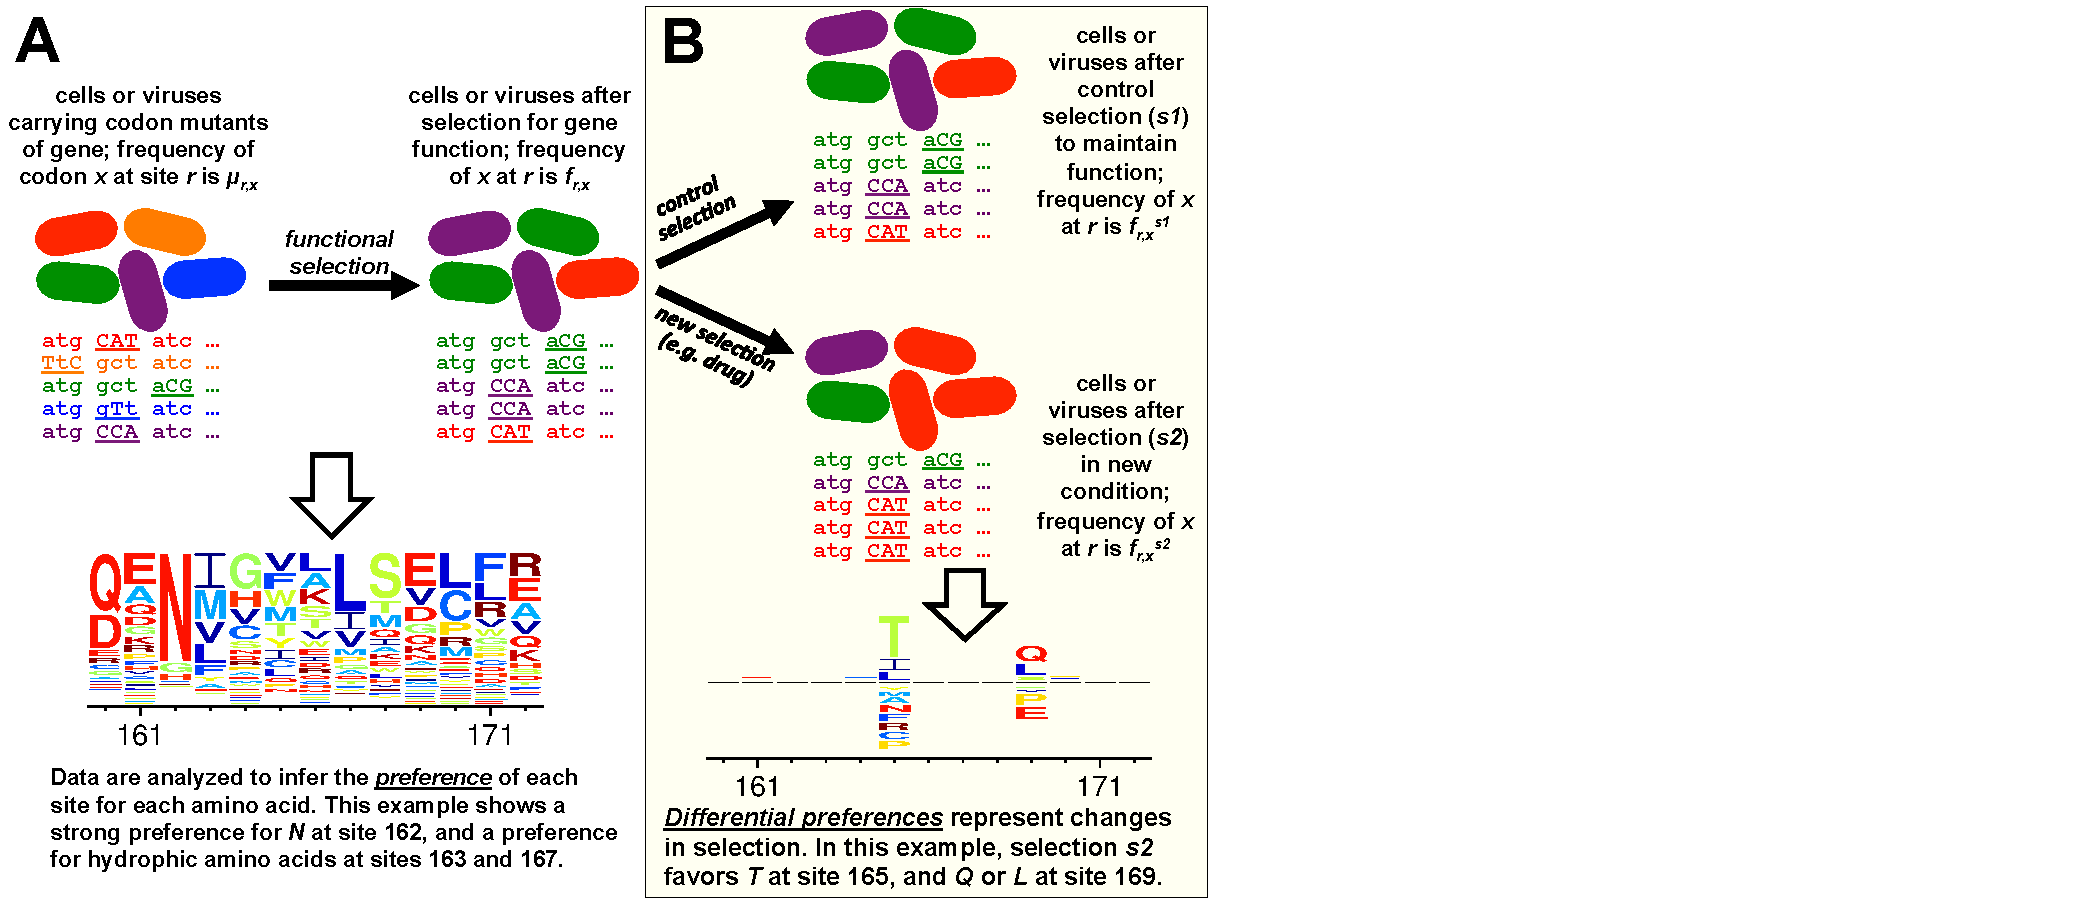
\includegraphics[clip, trim=0in 0in 5.92in 0in, width=5.5in]{Fig_DeepMutationalScan/Fig_DeepMutationalScan.pdf}}
\caption{\label{fig:DeepMutationalScan}{\csentence{A deep mutational scanning experiment.} {\bf (A)} A gene is mutagenized to create a library that contains all single codon mutations. The mutant library is introduced into cells or viruses and subjected to a functional selection that enriches beneficial mutations and depletes deleterious ones. Deep sequencing is used to count mutations in a sample of the variants present pre- and post-selection. Using \texttt{dms\_tools}, the data can be analyzed to infer the ``preference'' of each site for each amino acid; in the visualization, letter heights are proportional to the preference for that amino acid. {\bf (B)} The experiment can be extended by subjecting the library of functional variants to two different selection pressures, and using deep sequencing to assess which variants are favored in one condition versus the other. Using \texttt{dms\_tools}, the data can be analyzed to infer the ``differential preference'' of each site for each amino acid in the alternative selection $s2$ versus the control selection $s1$; in the visualization, letter heights above or below the line are proportional to the differential preference for or against that amino acid.}}
\end{figure}

\begin{figure}[h!]
\centerline{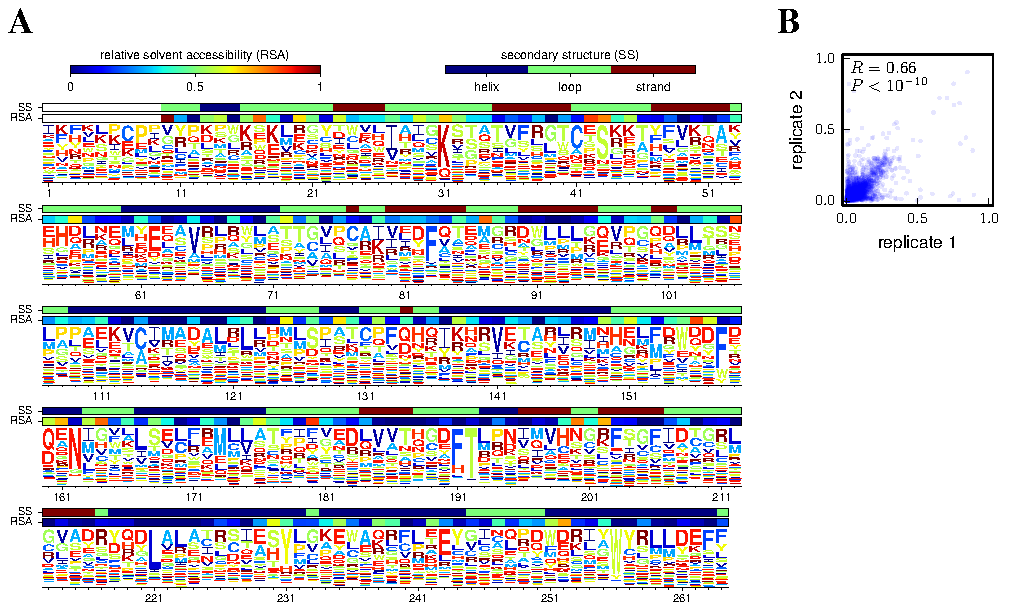
\includegraphics[width=6.7in]{Fig_MelnikovPrefs/Fig_MelnikovPrefs.pdf}}
\cprotect \caption{\label{fig:MelnikovPrefs}\csentence{Site-specific preferences from deep mutational scanning of a Tn5 transposon.} Melnikov \textit{et al}~\cite{melnikov2014comprehensive} performed deep mutational scanning on a Tn5 transposon using kanamycin selection, and reported the counts of amino-acid mutations for two biological replicates of the experiment. Here I have used \texttt{dms\_tools} to infer the preferences. {\bf (A)} Visualization of the preferences averaged across the two replicates. {\bf (B)} Correlation between the preferences inferred from each of the two replicates. Given files containing the mutation counts, the plots can be generated as \texttt{logoplot.pdf} and \texttt{corr.pdf} with the following commands:
\begin{lstlisting} 
dms_inferprefs pre_counts_1.txt post_counts_1.txt prefs_1.txt --excludestop --ncpus -1 --chartype aa
dms_inferprefs pre_counts_2.txt post_counts_2.txt prefs_2.txt --excludestop --ncpus -1 --chartype aa
dms_correlate prefs_1.txt prefs_2.txt corr --name1 "replicate 1" --name2 "replicate 2" --corr_on_plot
dms_merge prefs.txt average prefs_1.txt prefs_2.txt
dms_logoplot prefs.txt logoplot.pdf --nperline 53 --overlay1 RSAs.txt RSA "relative solvent accessibility" --overlay2 SSs.txt SS "secondary structure"
\end{lstlisting}
}
\end{figure}

\begin{figure}[h!]
\centerline{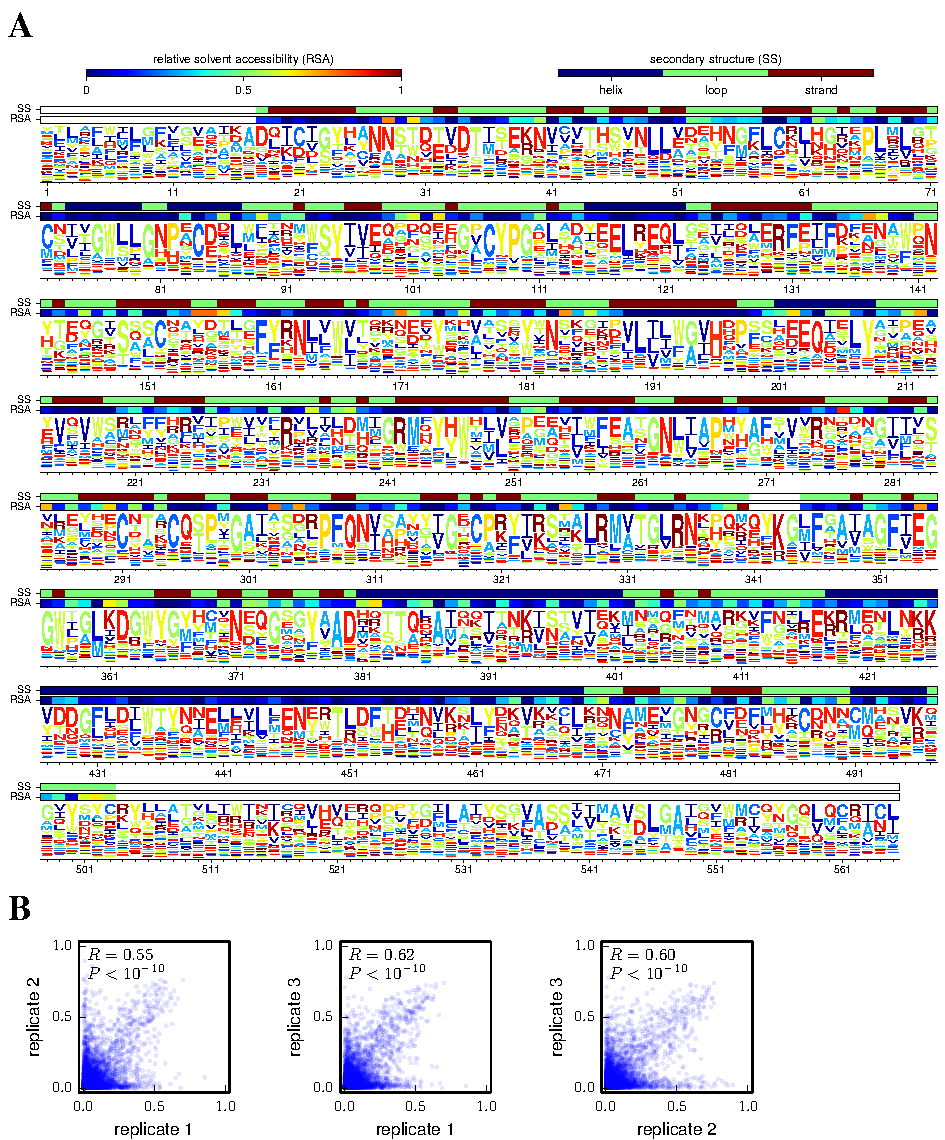
\includegraphics[width=6.1in]{Fig_ThyagarajanPrefs/Fig_ThyagarajanPrefs.pdf}}
\cprotect \caption{\label{fig:ThyagarajanPrefs}\csentence{Site-specific preferences from deep mutational scanning of influenza hemagglutinin.} Thyagarajan and Bloom~\cite{thyagarajan2014inherent} performed deep mutational scanning on influenza hemagglutinin, and reported the counts of codon mutations for three biological replicates of the experiment. Here I have used \texttt{dms\_tools} to infer the preferences. {\bf (A)} Visualization of the preferences averaged across the three replicates. {\bf (B)} Correlations between the preferences from each pair of replicates. Given files containing the mutation counts, the plots can be generated as \texttt{logoplot.pdf}, \texttt{corr\_1\_2.pdf}, \texttt{corr\_1\_3.pdf}, and \texttt{corr\_2\_3.pdf} with the following commands:
\begin{lstlisting} 
dms_inferprefs mutDNA_1.txt mutvirus_1.txt prefs_1.txt --errpre DNA_1.txt --errpost virus_1.txt --ncpus -1
dms_inferprefs mutDNA_2.txt mutvirus_2.txt prefs_2.txt --errpre DNA_2.txt --errpost virus_2.txt --ncpus -1
dms_inferprefs mutDNA_3.txt mutvirus_3.txt prefs_3.txt --errpre DNA_3.txt --errpost virus_3.txt --ncpus -1
dms_correlate prefs_1.txt prefs_2.txt corr_1_2 --name1 "replicate 1" --name2 "replicate 2" --corr_on_plot
dms_correlate prefs_1.txt prefs_3.txt corr_1_3 --name1 "replicate 1" --name2 "replicate 3" --corr_on_plot
dms_correlate prefs_2.txt prefs_3.txt corr_2_3 --name1 "replicate 2" --name2 "replicate 3" --corr_on_plot
dms_merge prefs.txt average prefs_1.txt prefs_2.txt prefs_3.txt
dms_logoplot prefs.txt logoplot.pdf --nperline 71 --overlay1 RSAs.txt RSA "relative solvent accessibility" --overlay2 SSs.txt SS "secondary structure" --excludestop
\end{lstlisting}
}
\end{figure}
      
\begin{figure}[h!]
\centerline{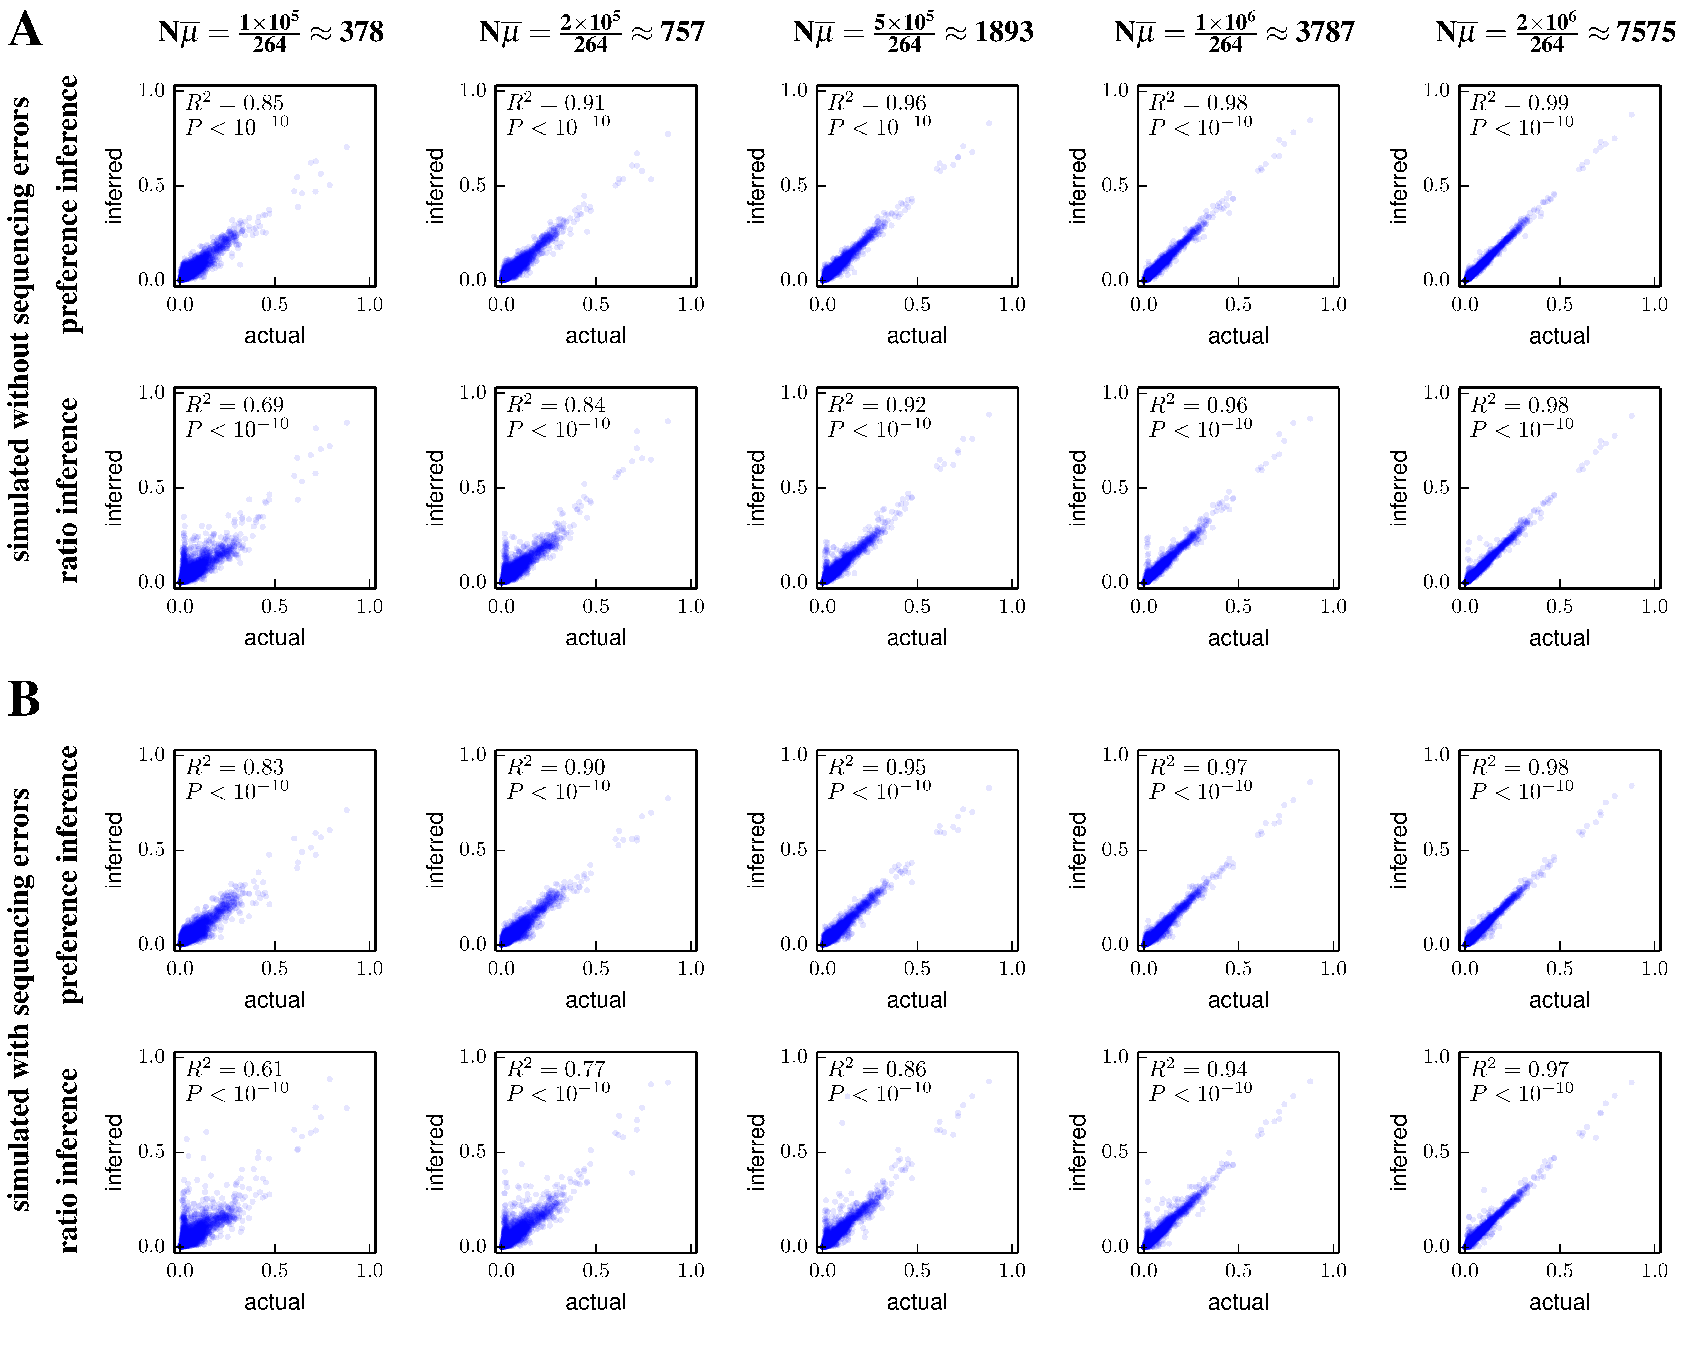
\includegraphics[width=6.5in]{../../examples/Melnikov_et_al_Tn5/infer_prefs_on_simulated_data/correlations.pdf}}
\cprotect\caption{\label{fig:PrefCorrelations}\csentence{Accuracy of preference inference on simulated data.} Deep mutational scanning counts were simulated using the preferences in Figure \ref{fig:MelnikovPrefs}A and realistic parameters for mutation and error rates. The simulations were done {\bf (A)} without or {\bf (B)} with sequencing errors quantified by control libraries. Plots show the correlation between the actual and inferred preferences as a function of the product of the sequencing depth $N$ and the average per-site mutation rate $\overline{\mu}$; real experiments typically have $N\overline{\mu} \sim 1000$ to 2000 depending on the sequencing depth and gene length. Preferences are inferred using the full algorithm in \texttt{dms\_tools} (top panels) or by simply calculating ratios of counts (bottom panels) using Equation \ref{eq:enrichmentcounts} and its logical extension to include errors, both with a pseudocount of one. The \texttt{dms\_tools} inferences are more accurate than the simple ratio estimation, with both methods converging to the actual values with increasing $N\overline{\mu}$. Given files with the mutation counts, the plots in this figure can be generated as \texttt{prefs\_corr.pdf} and \texttt{ratio\_corr.pdf} with commands such as:
\begin{lstlisting}
dms_inferprefs pre.txt post.txt inferred_prefs.txt --ncpus -1
dms_inferprefs pre.text post.text ratio_prefs.txt --ratio_estimation 1
dms_correlate actual_prefs.txt inferred_prefs.txt prefs_corr --name1 "actual" --name2 "inferred" --corr_on_plot --r2
dms_correlate actual_prefs.txt ratio_prefs.txt ratio_corr --name1 "actual" --name2 "inferred" --corr_on_plot --r2
\end{lstlisting}
}
\end{figure}

\begin{figure}[h!]
\centerline{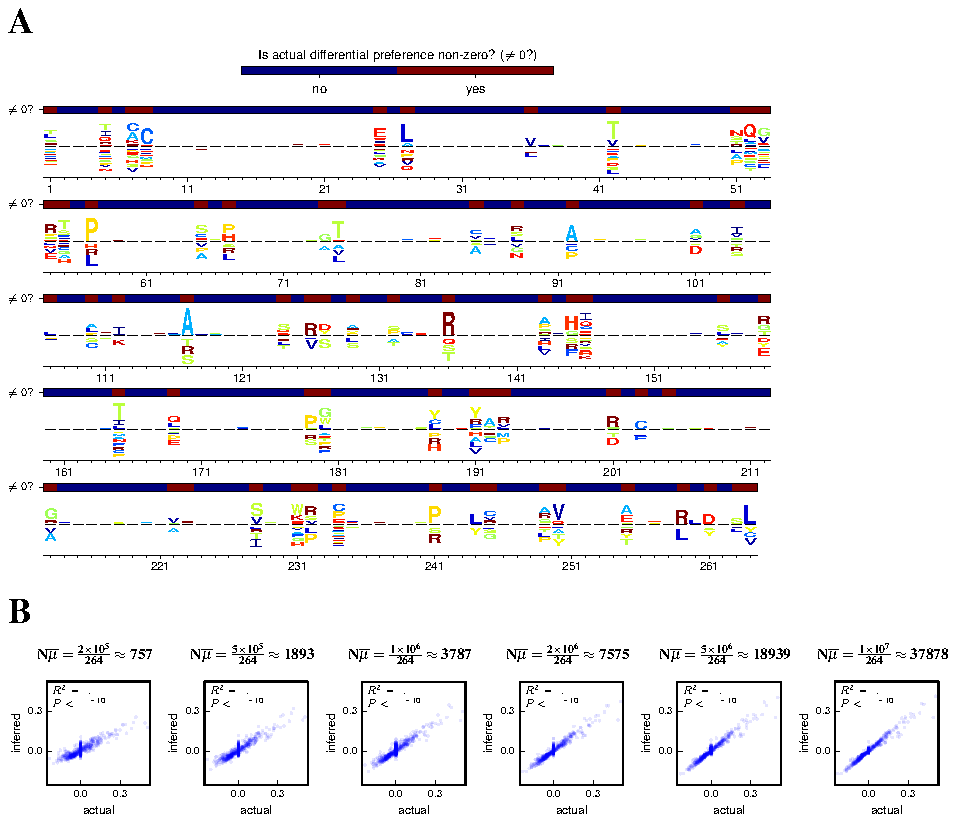
\includegraphics[width=6.5in]{Fig_MelnikovDiffPrefs/Fig_MelnikovDiffPrefs.pdf}}
\cprotect\caption{\label{fig:MelnikovSimulatedDiffPrefs}\csentence{Inference of differential preferences on simulated data.} To illustrate and test the inference of differential preferences, the experiment in Figure \ref{fig:DeepMutationalScan}B was simulated at the codon level starting with the post-selection library that yielded the preferences in Figure \ref{fig:MelnikovPrefs}. In the simulations, 20\% of sites had different preferences between the control and alternative selection. {\bf (A)}, \texttt{dms\_tools} was used to infer the differential preferences from the data simulated at $N = 10^7$, and the resulting inferences were visualized. The overlay bars indicate which sites had non-zero differential preferences in the simulation. {\bf (B)} The correlations between the inferred and actual differential preferences as a function of $N\overline{\mu}$ show that the inferred values converge to the true ones. Given files with the mutation counts, the plots in this figure can be generated as \texttt{logoplot.pdf} and \texttt{corr.pdf} with the following commands:
\begin{lstlisting}
dms_inferdiffprefs start.txt s1.txt s2.txt diffprefs.txt --ncpus -1 
dms_logoplot diffprefs.txt  logoplot.pdf --nperline 53 --overlay1 actually_nonzero.txt "$\ne 0$?" "Is actual differential preference non-zero?" --diffprefheight 0.45
dms_correlate actual_diffprefs.txt diffprefs.txt corr --name1 "actual" --name2 "inferred" --corr_on_plot --r2
\end{lstlisting}
}
\end{figure}

\begin{figure}[h!]
\centerline{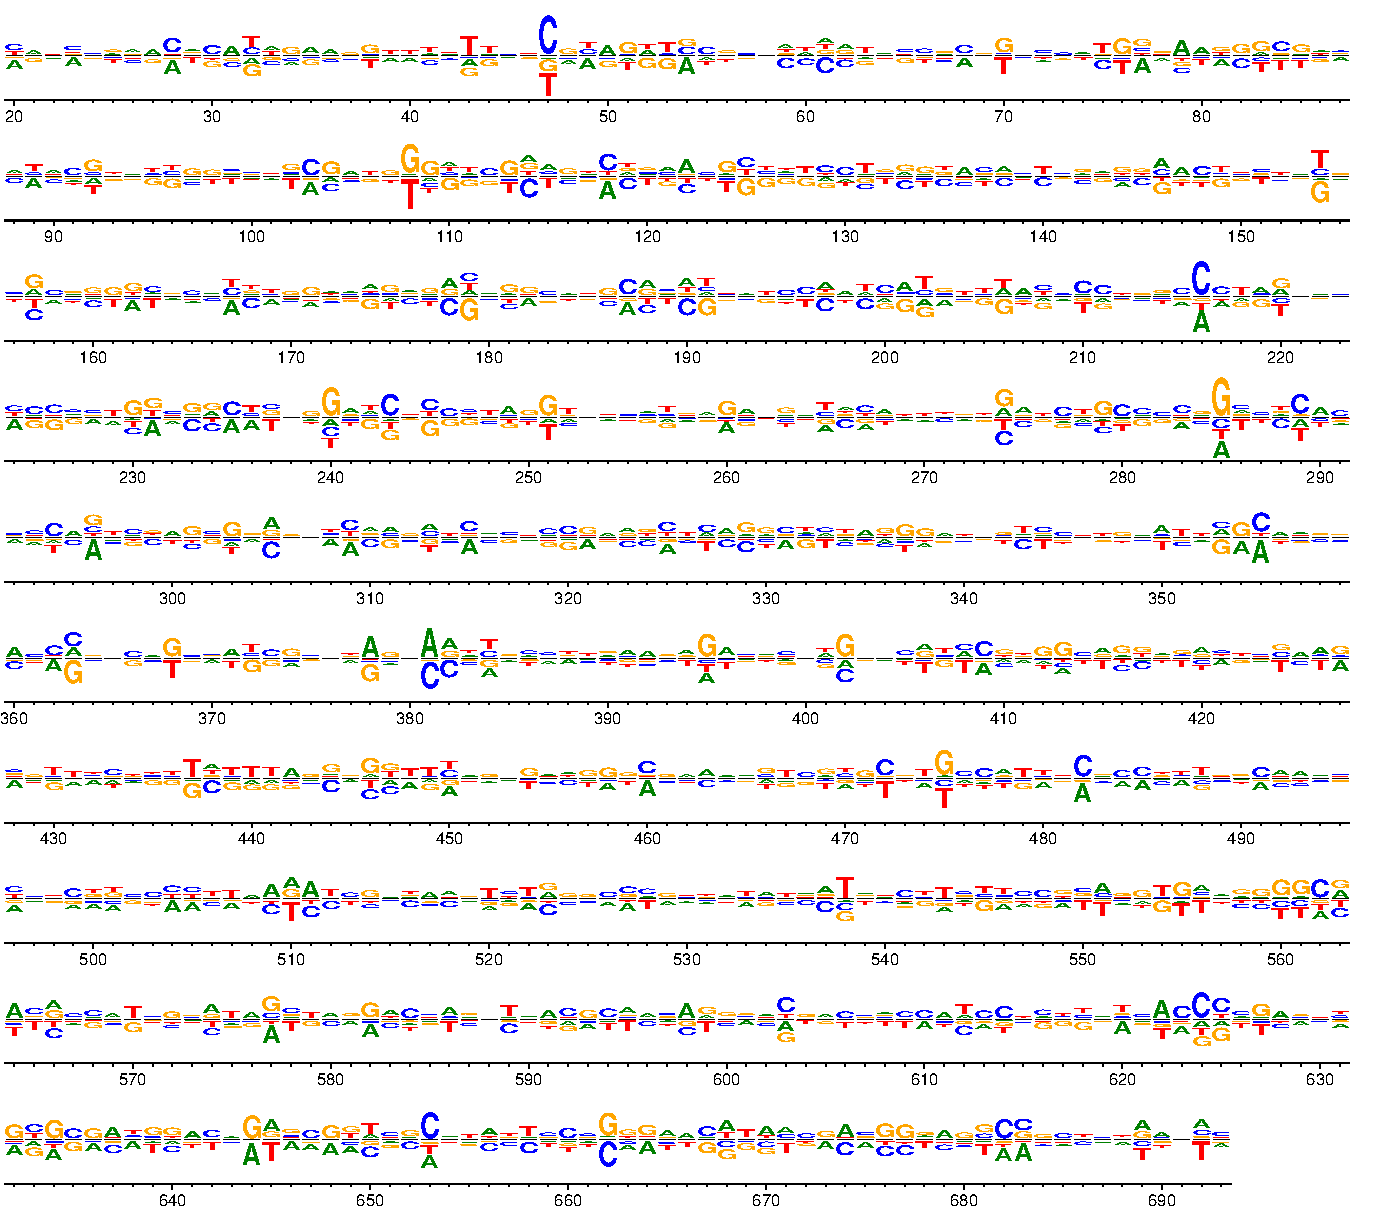
\includegraphics[width=6.5in]{../../examples/Wu_et_al_NS1/diffprefs_logoplot.pdf}}
\cprotect\caption{\label{fig:WuDiffPrefs}\csentence{Differential preferences following selection of influenza NS1 in the presence or absence of interferon.} Wu \textit{et al}~\cite{wu2014ns} generated libraries of influenza viruses carrying nucleotide mutations in the NS segment. They passaged these viruses in the presence or absence of interferon pre-treatment. Here, \texttt{dms\_tools} was used to analyze and visualize the data to identify sites where different nucleotides are preferred in the presence versus the absence of interferon. Because the mutations were made at the nucleotide level, the data must also be analyzed at that level (unlike in Figures \ref{fig:MelnikovPrefs}, \ref{fig:ThyagarajanPrefs}, and \ref{fig:MelnikovSimulatedDiffPrefs}, where codon mutagenesis means that the data can be analyzed at the amino-acid level). The plot can be generated as \texttt{logoplot.pdf} with the following commands:
\begin{lstlisting}
dms_inferdiffprefs input.txt control.txt interferon.txt diffprefs.txt --ncpus -1 --chartype DNA
dms_logoplot diffprefs.txt logoplot.pdf --nperline 68 --diffprefheight 0.4
\end{lstlisting}
}
\end{figure}

%%%%%%%%%%%%%%%%%%%%%%%%%%%%%%%%%%%
%%                               %%
%% Tables                        %%
%%                               %%
%%%%%%%%%%%%%%%%%%%%%%%%%%%%%%%%%%%

%% Use of \listoftables is discouraged.
%%


%%%%%%%%%%%%%%%%%%%%%%%%%%%%%%%%%%%
%%                               %%
%% Additional Files              %%
%%                               %%
%%%%%%%%%%%%%%%%%%%%%%%%%%%%%%%%%%%



\end{backmatter}
\end{document}
